\chapter{Introduction}
Radio astronomers are trying to answer a very diverse set of questions. 

%Are we alone?
%When were the first stars and galaxies formed?
%Galactic structure and formation (mapping the galaxy)
%Nature of gravitational wave background (pulsar timing)
%Transient universe
%Black hole imaging
%Searching for extrasolar planets


\section{Motivation}

%TODO: Make this prettier
\begin{figure}[ht!]
  \centering
    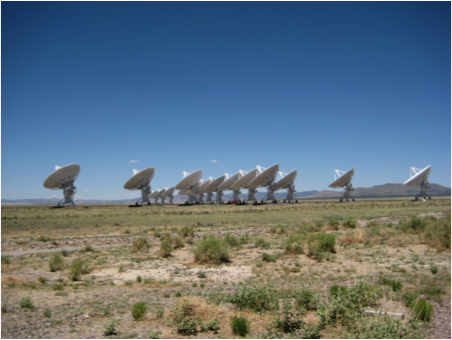
\includegraphics[height=0.35\textheight]{Images/C1/vla.png}
    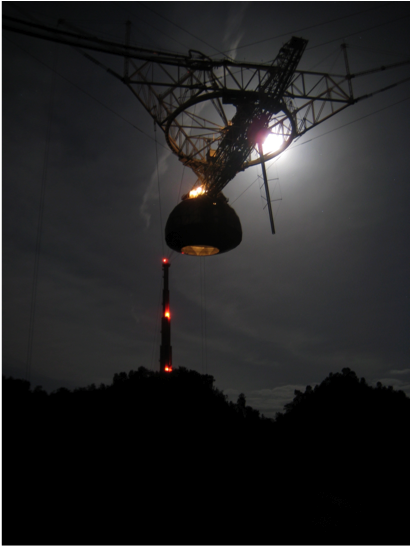
\includegraphics[height=0.35\textheight]{Images/C1/arecibo.png}
    %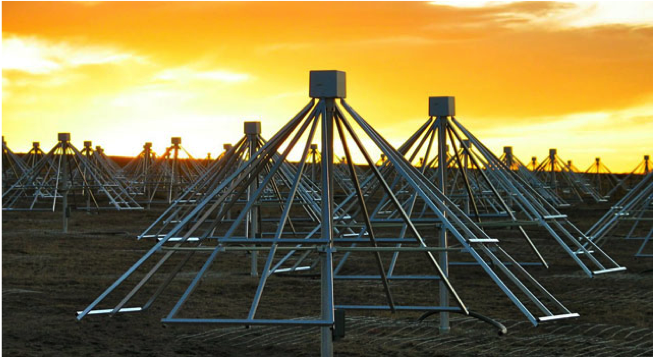
\includegraphics[width=0.49\textwidth]{Images/C1/paper.png}
  \caption[The VLA and Arecibo Telescopes]{The VLA and Arecibo Telescopes}
  \label{fig: C1/telescopes}
\end{figure}


%TODO: Make this prettier, maybe add a graphic
%\begin{figure}[ht!]
%  \centering
%    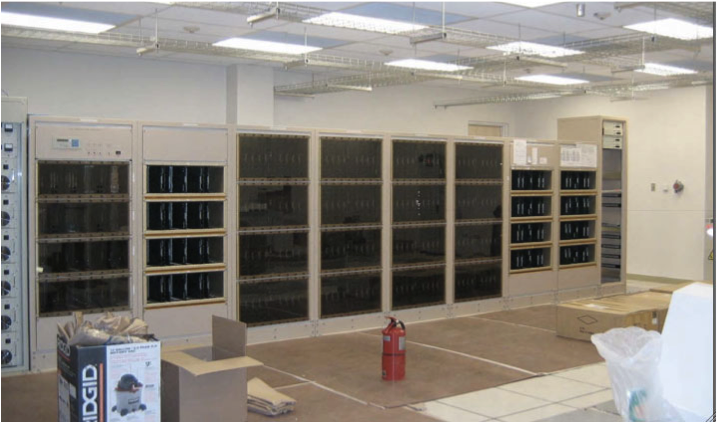
\includegraphics[width=0.49\textwidth]{Images/C1/alma_correlator.png}
%    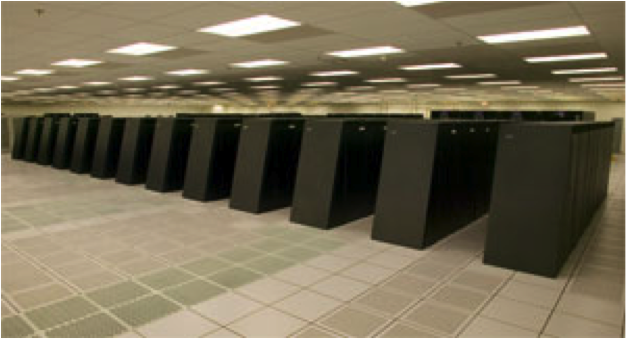
\includegraphics[width=0.49\textwidth]{Images/C1/blue_gene.png}
%    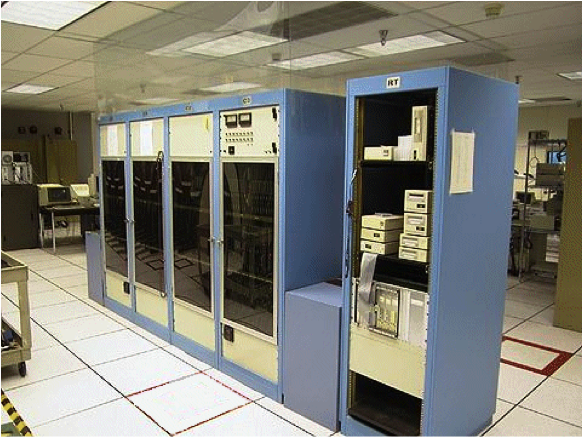
\includegraphics[width=0.49\textwidth]{Images/C1/vla_correlator.png}
%  \caption{TODO Building large systems}
%  \label{fig: C1/largesystems}
%\end{figure}

%TODO: add some references

%\begin{figure}[ht!]
%  \centering
%    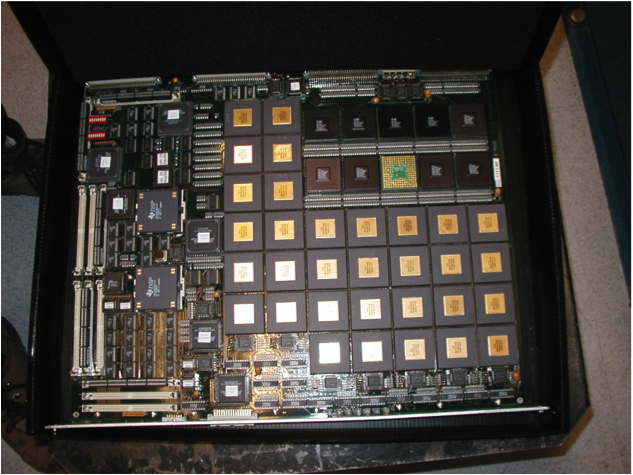
\includegraphics[width=0.49\textwidth]{Images/C1/custom_asic.png}
%    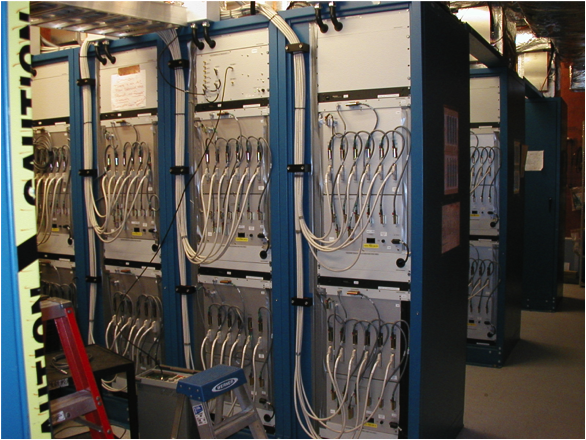
\includegraphics[width=0.49\textwidth]{Images/C1/custom_interconnect.png}
%  \caption{TODO Building large systems}
%  \label{fig: C1/largesystems}
%\end{figure}


Traditionally, observatories designed custom instruments that would run on one telescope and solve one problem.
This custom approach was the only way to get the requisite processing power to analyze the radio signals, but it resulted in costly designs, because the boards, backplanes, chips, protocols, and software all needed to be designed from scratch.
To make matters worse, this approach resulted in a very long design cycle,  requiring 5-10 years of development before an instrument could be deployed at a telescope and the time the instrument was released, the hardware would be out of date.

Due to their custom implementations, these instruments also lacked flexibility. 
Each instrument was designed specifically for a single purpose.
A hardware upgrade or algorithm modification would require a complete redesign of the instrument, and another long design cycle.

While these older designs needed to trade off flexibility for performance, newer technology can offer both performance and flexibility.
Programmable devices such as FPGAs, GPUs and even CPUs can provide enough processing power to keep up with the data from many new telescopes.
These devices make it easy to reprogram existing hardware to support newer algorithms, and, since they are programmed using portable languages, provide a quick path to upgrade hardware without redesigning the entire instrument.

With a huge range of technology available, choosing what hardware to use to build an instrument is a challenge. 

\section{Challenges}


\subsection{Scientific Challenges}

%Number of antennas
%Bandwidth
%Number of channels
%Filter shapes
%Integration time
%Algorithms
%Etc�

%Spectrometer
%Beamformer
%Add signals from multiple antennas together to improve SNR
%Pulsar processor
%Detect dispersed pulse
%Interferometer/correlator
%Cross-correlate signals from many antennas to combine into a spectral image
%Increase angular resolution

%Spectrometer
%Filter bank/FFT
%Accumulation
%Beamformer
%FFT
%Phase shift
%Adders
%Pulsar processor
%FFT
%Deconvolution
%Interferometer/correlator
%FFT
%Cross correlation (multipliers)
%Accumulation

%Large number of small antennas to improve sensitivity and resolution
%Small antennas are very low cost
%Creates very high performance signal processing requirements
%Need to combine the antennas together to form a single image or beam
%Interferometry computation requirements scale as N2 (N = number of antennas) ~100Tops

\subsection{Technological Challenges}

When building a large instrument, there is a wide variety of technology to choose from.
Unlike many applications, where the goal is to provide the fastest possible implementation, in real time radio astronomy instrumentation there is a performance target.
 Understanding the tradeoffs between different implementations is key to cost-effective design.

\begin{figure}[ht!]
  \centering
    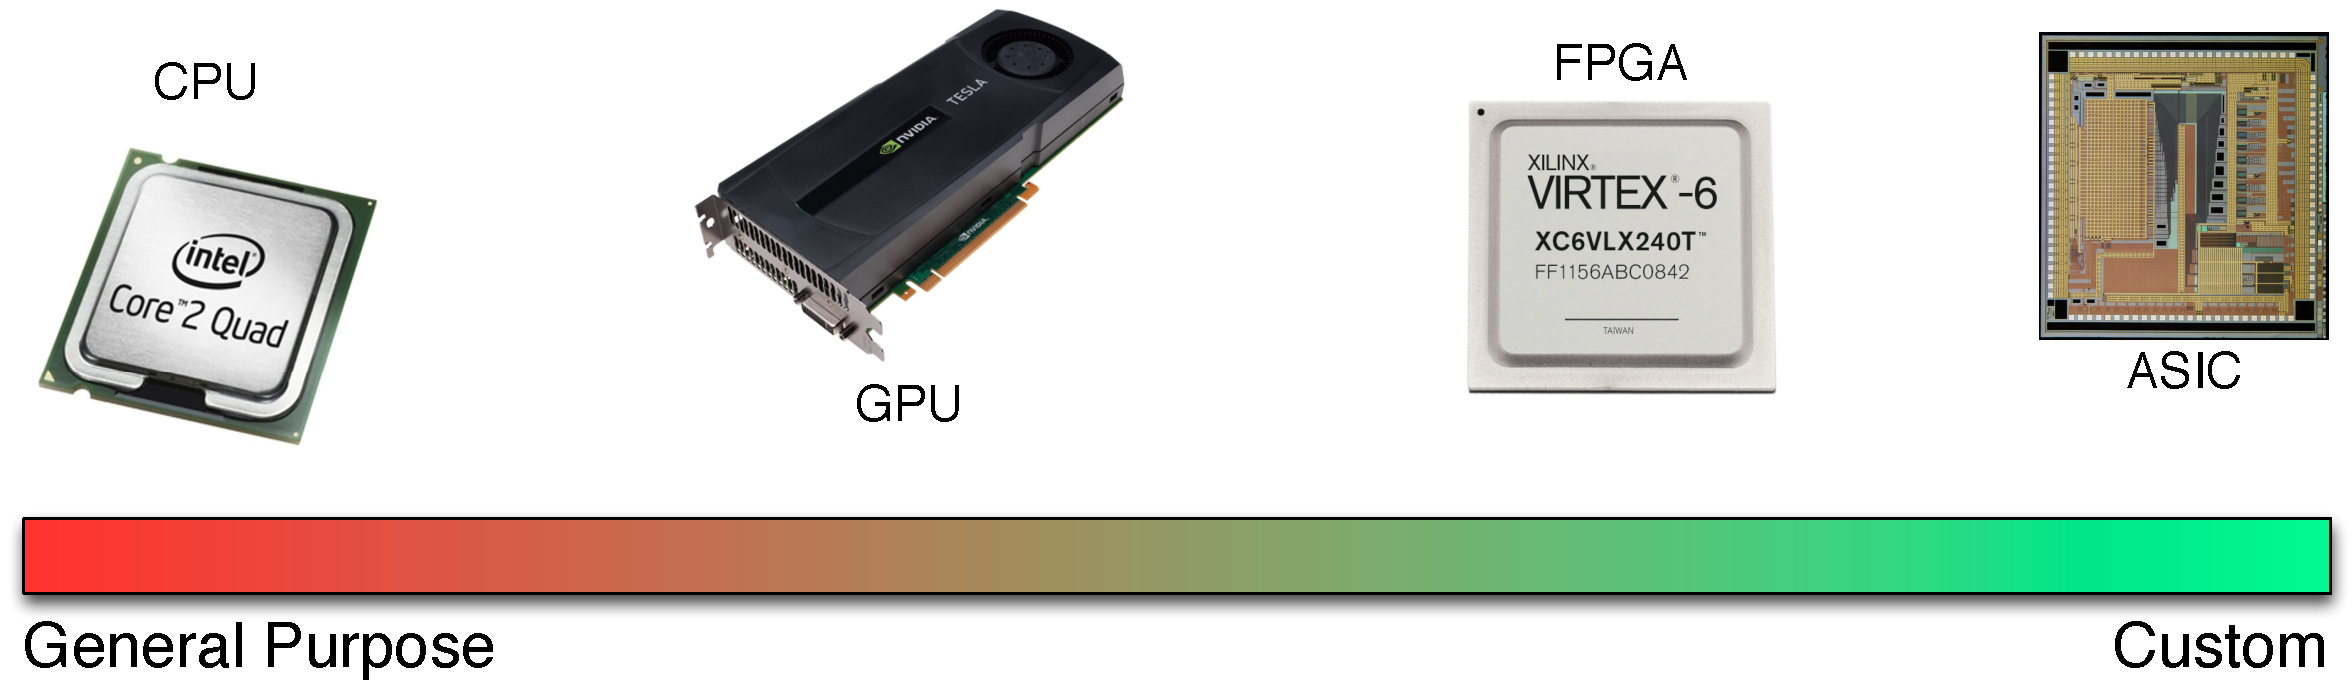
\includegraphics[width=\textwidth]{Images/C1/design_space.pdf}
  \caption{Technology Spectrum}
  \label{fig: C1/design_space.pdf}
\end{figure}

An instrument designed typically has four choices of hardware for their algorithm implementations. 
They can use CPUs, GPUs, FPGAs, and ASICs.
Figure \ref{fig: C1/design_space.pdf} shows each of these as a spectrum from general purpose to custom.
The CPUs and, to a lesser extend GPUs, provide a very general purpose design experience, while FPGAs and ASICs require custom designs.
This spectrum also can be used to generalize a number of other properties of the presented hardware.
Platforms further right require higher design times and design complexity and less flexibility in the final design.
And because the chips will be deployed in relatively low volume, the platforms on the right will also cost more money. 
The tradeoff is in power and performance. 
The benefit that comes with the platforms on the left is higher performance and lower power consumption. 

To better understand these tradeoffs, I compare the two platforms in the center of the spectrum, the GPU and FPGA.
NVIDIA GPUs can be programmed in CUDA.
It's C-like structure makes it easy for CPU programmers to pick up and provides a lot of flexibility. 
CUDA allows the programmer to use conditional and Iterative programming the same way they would use C, easing the transition into GPU programming.
FPGAs are programmed using a hardware description language, or HDL, which is less flexible and harder to learn than CUDA.
In the FPGA computing model the data is streaming and everything is happening at the same time, requiring specialized programming.
%TODO: discuss C-to-gates
On the other hand, FPGAs offer an order of magnitude improvement in performance and power consumption.
Each GPU requires hundreds of watts of power while an FPGA can be powered with tens of watts and a GPU can only process hundreds of megahertz of antenna data while an FPGA is capable of processing multiple gigahertz.

Although it may be easy to enumerate the differences between these platforms, understanding which is best is more difficult.
In most cases, a heterogeneous approach is best, 
The best mix of platforms will ultimately depend on the desired instrument, available technology, as well as the price and power restrictions.
This means that a brand new implementation must be designed for every new instrument.


\section{Optimal Rearrangement of Cluster-based Astronomy Signal Processing}
This dissertation explores an automated approach to instrument design using a tool called Optimal Rearrangement of Cluster-based Astronomy Signal Processing or ORCAS.
This tool was designed to provide cost-optimal mappings in a short amount of time.
ORCAS allows the developer to define the instrument at a high level and a cost function defining some cost the developer is aiming to minimize.
The cost function can represent something as simple as the price of the instrument or can be used to represent more complex parameters of the instrument such as design time.

ORCAS assesses the performance of different types of technologies in two ways.
First, by using benchmarks of existing implementations of instrument building blocks such as FFTs and FIR filters we can directly assess the performance.
Second, if a benchmark is not available, the tool can use a performance model instead, giving an estimate of how the block will perform.
This makes it easy to keep up with improving technology and library performance without rewriting the entire tool every time a new library version or board is released. 

We evaluate ORCAS by benchmarking existing libraries, such as CUFFT and the CASPER library, and use those benchmarks to produce mappings for 3 types of instruments.
Each mapping is compared to existing implementations to understand how this automated approach compares to the old approach of hand optimized mapping.

The remainder of the dissertation is organized as follows.
Chapter \ref{chap:Real Time Radio Astronomy Algorithms} provides a more in-depth look at the algorithms commonly used in radio astronomy and their applications.
Chapter \ref{chap:Related Work} describes related work, done by myself and others, that preceded this work.
Chapter \ref{chap:High Level Toolflow} presents a high level description of the tool and explains how the tool goes from a description of the instrument to a fully mapped algorithm.
The algorithm used to map the instrument is fully specified in chapter \ref{chap:Algorithm Partitioning}.
Chapter \ref{chap:Analysis} describes three instrument case studies and compares them to existing instruments. 
And finally, in Chapter \ref{chap:Conclusions}, I present my conclusions and some opportunities for future work.






